\begin{frame}{Distribution of Track Parameters}
    \centering
    % \underline{Basic Plot Parameters}
    \begin{itemize}
        \item longTracks
        \item Track Propagation Error
        \item Track Chi2
        \item Track Chi2perDoF
        \item Track nDoF
        \item Track charge
        \item Track nLayers
    \end{itemize}
\end{frame}

\begin{frame}{Distribution of longTracks}
    \begin{figure}
        % 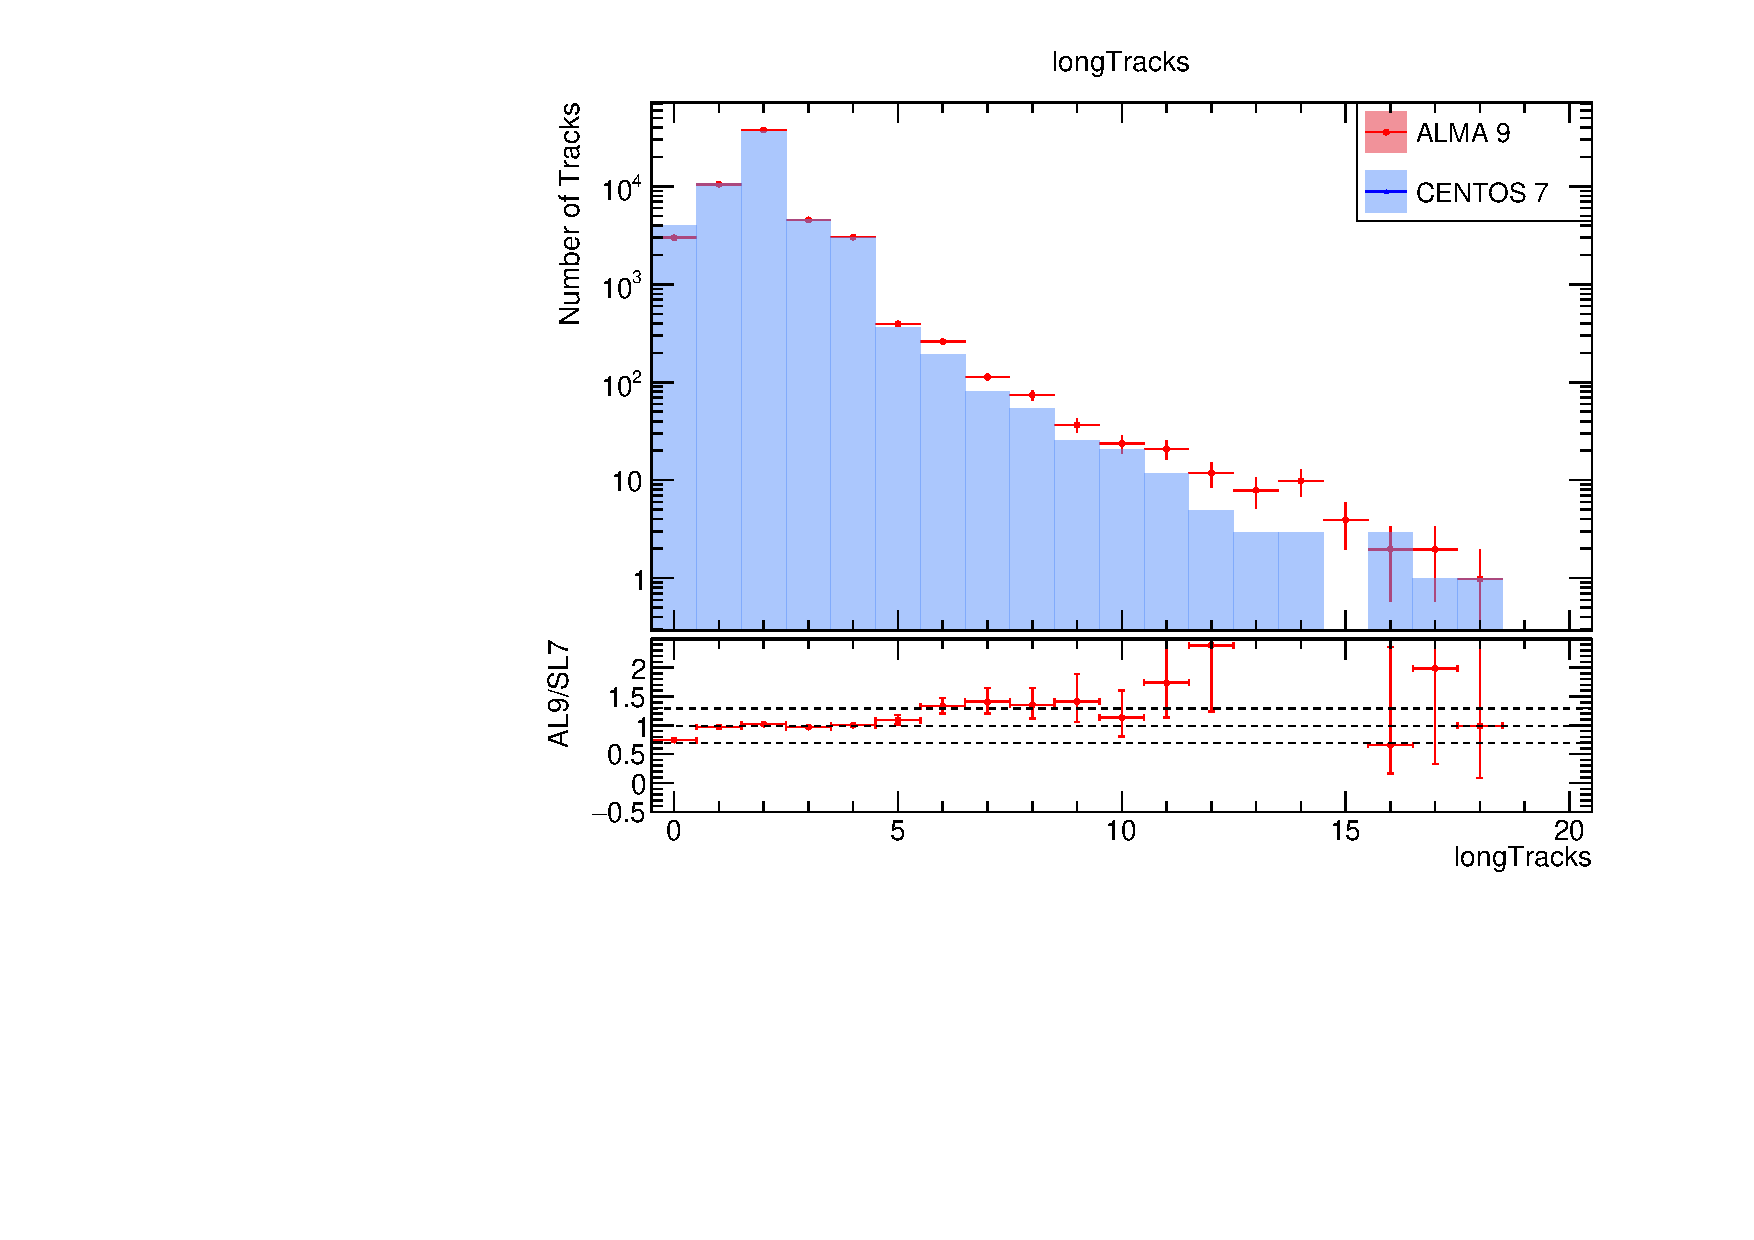
\includegraphics[width=\linewidth]{./output/longTracks.pdf}
        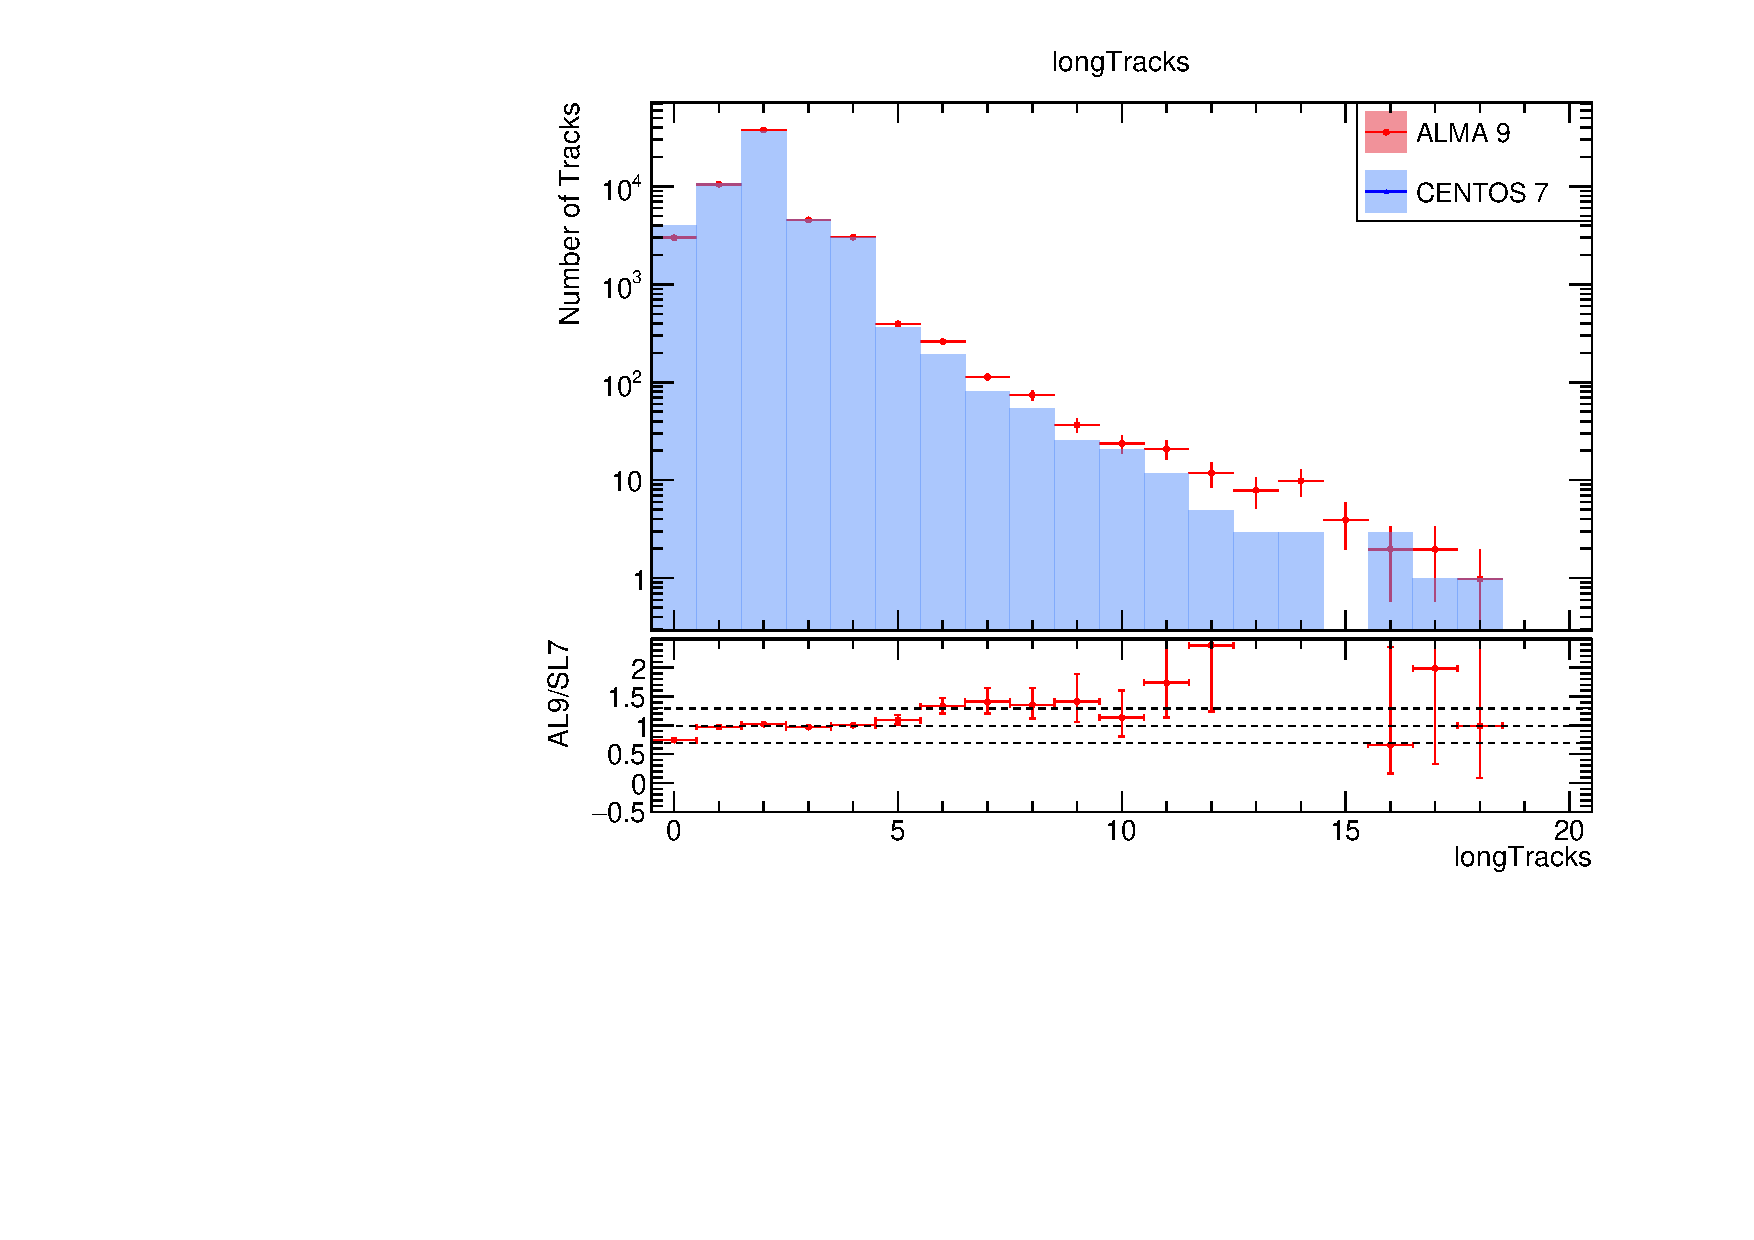
\includegraphics[width=\linewidth]{output/longTracks.pdf}
    \end{figure}
\end{frame}

\begin{frame}{Distribution of longTracks}
    \begin{tikzpicture}
        \node (img) {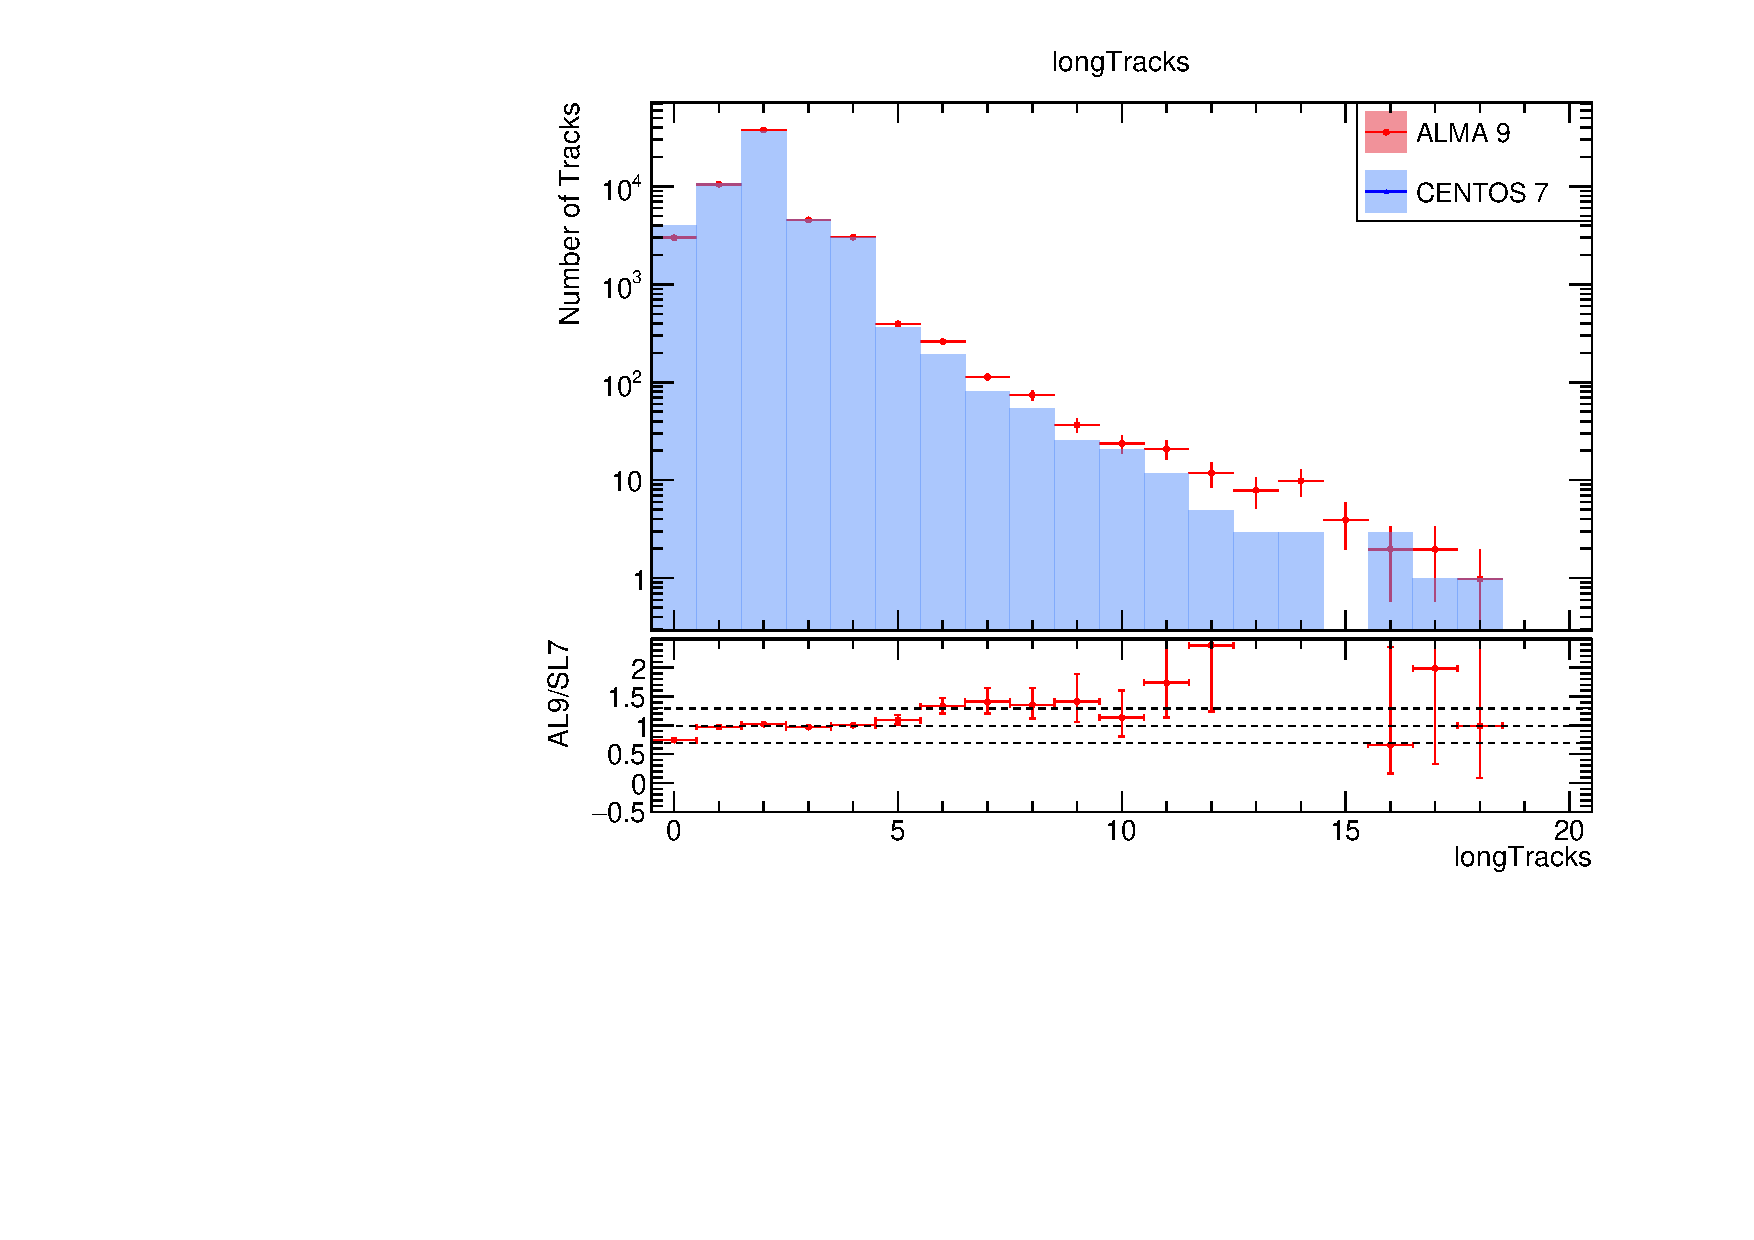
\includegraphics[width=\linewidth]{output/longTracks.pdf}};
        % \node [below left,text width=3cm,align=center] at (img.north east){Lorem ipsum dolor sit amet consectetur and then a bunch more stuff that no one remembers.\footnotemark};
        \node at (1.3, 1.5) {\color{red}{longTracks more than 5 is a mess}};
    \end{tikzpicture}

\end{frame}

\begin{frame}{Distribution of TrackPropagationError [SKIP]}
    \begin{figure}
        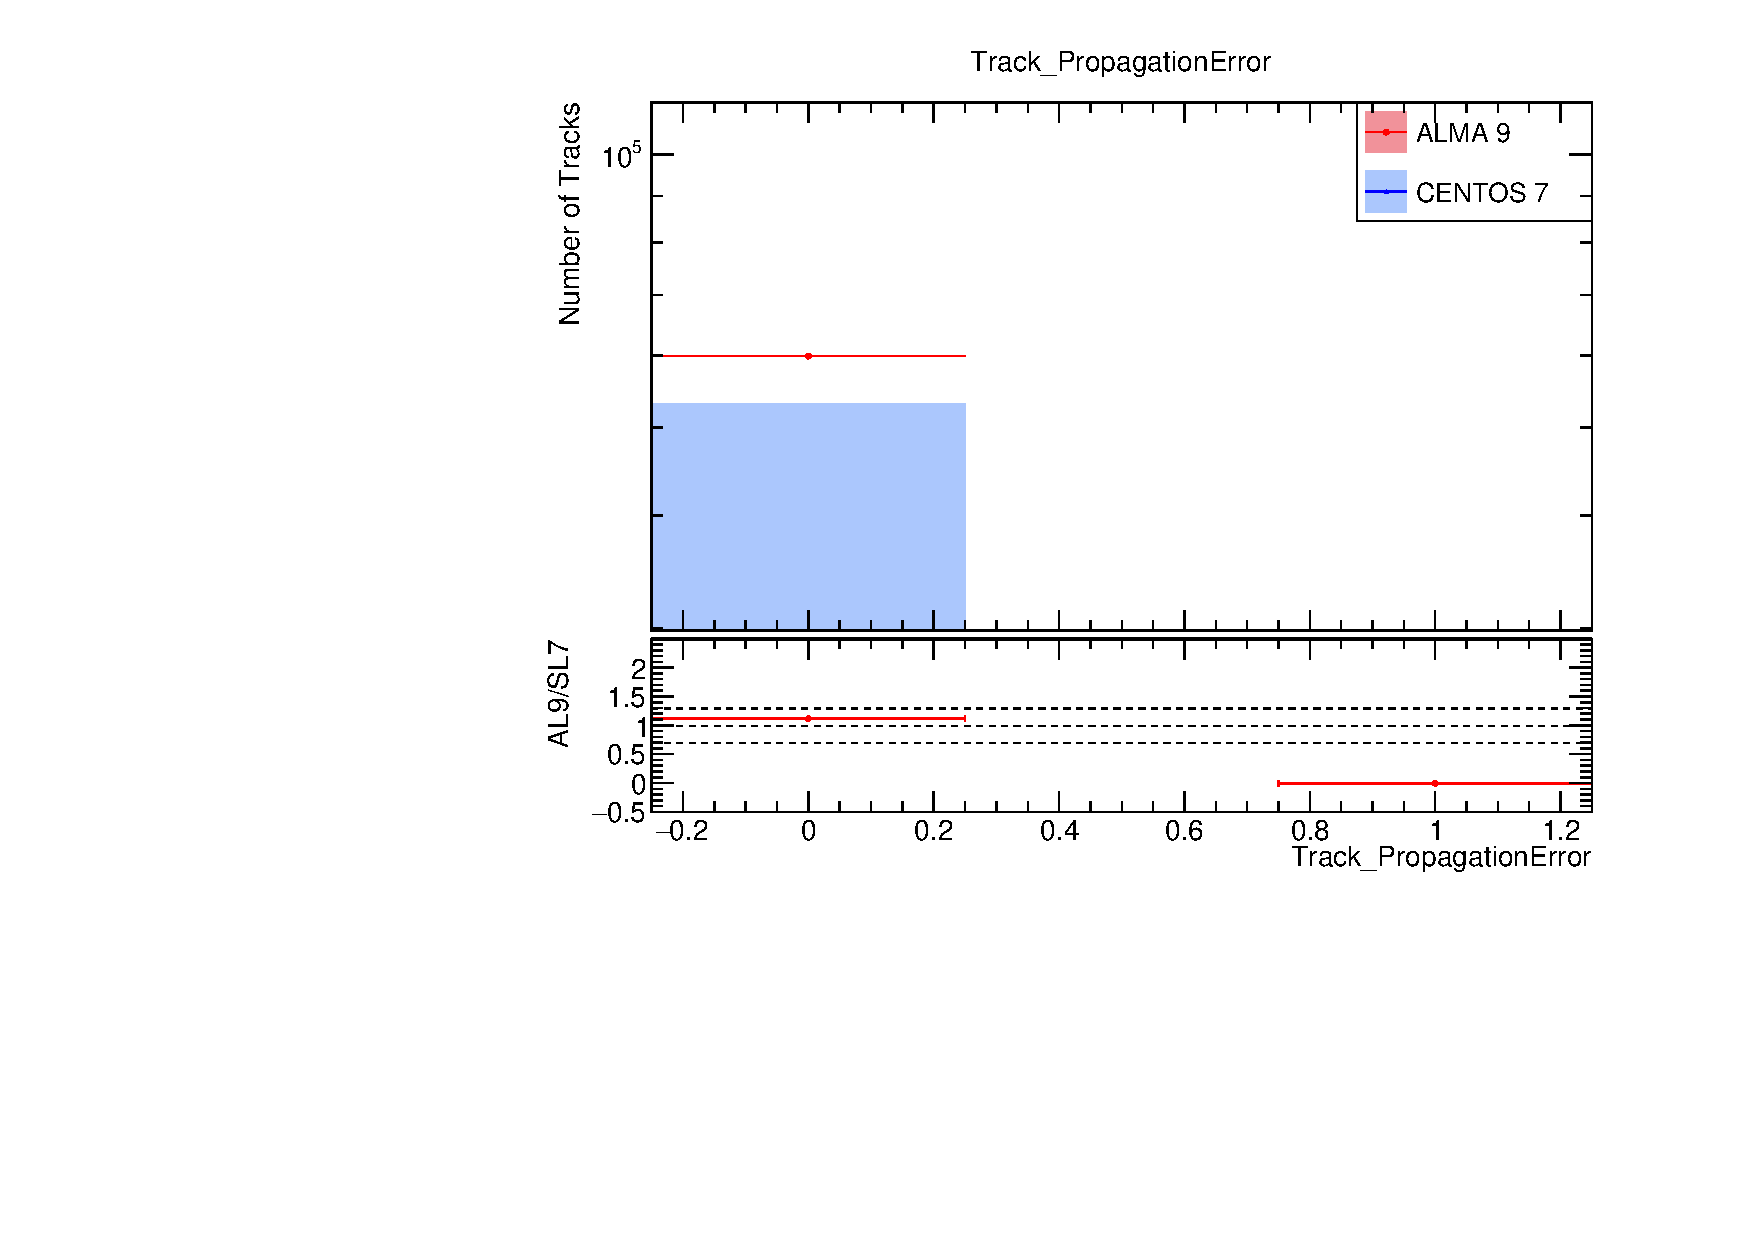
\includegraphics[width=\linewidth]{output/Track_PropagationError.pdf}
    \end{figure}
\end{frame}

\begin{frame}{Distribution of TrackChi2}
    \begin{figure}
        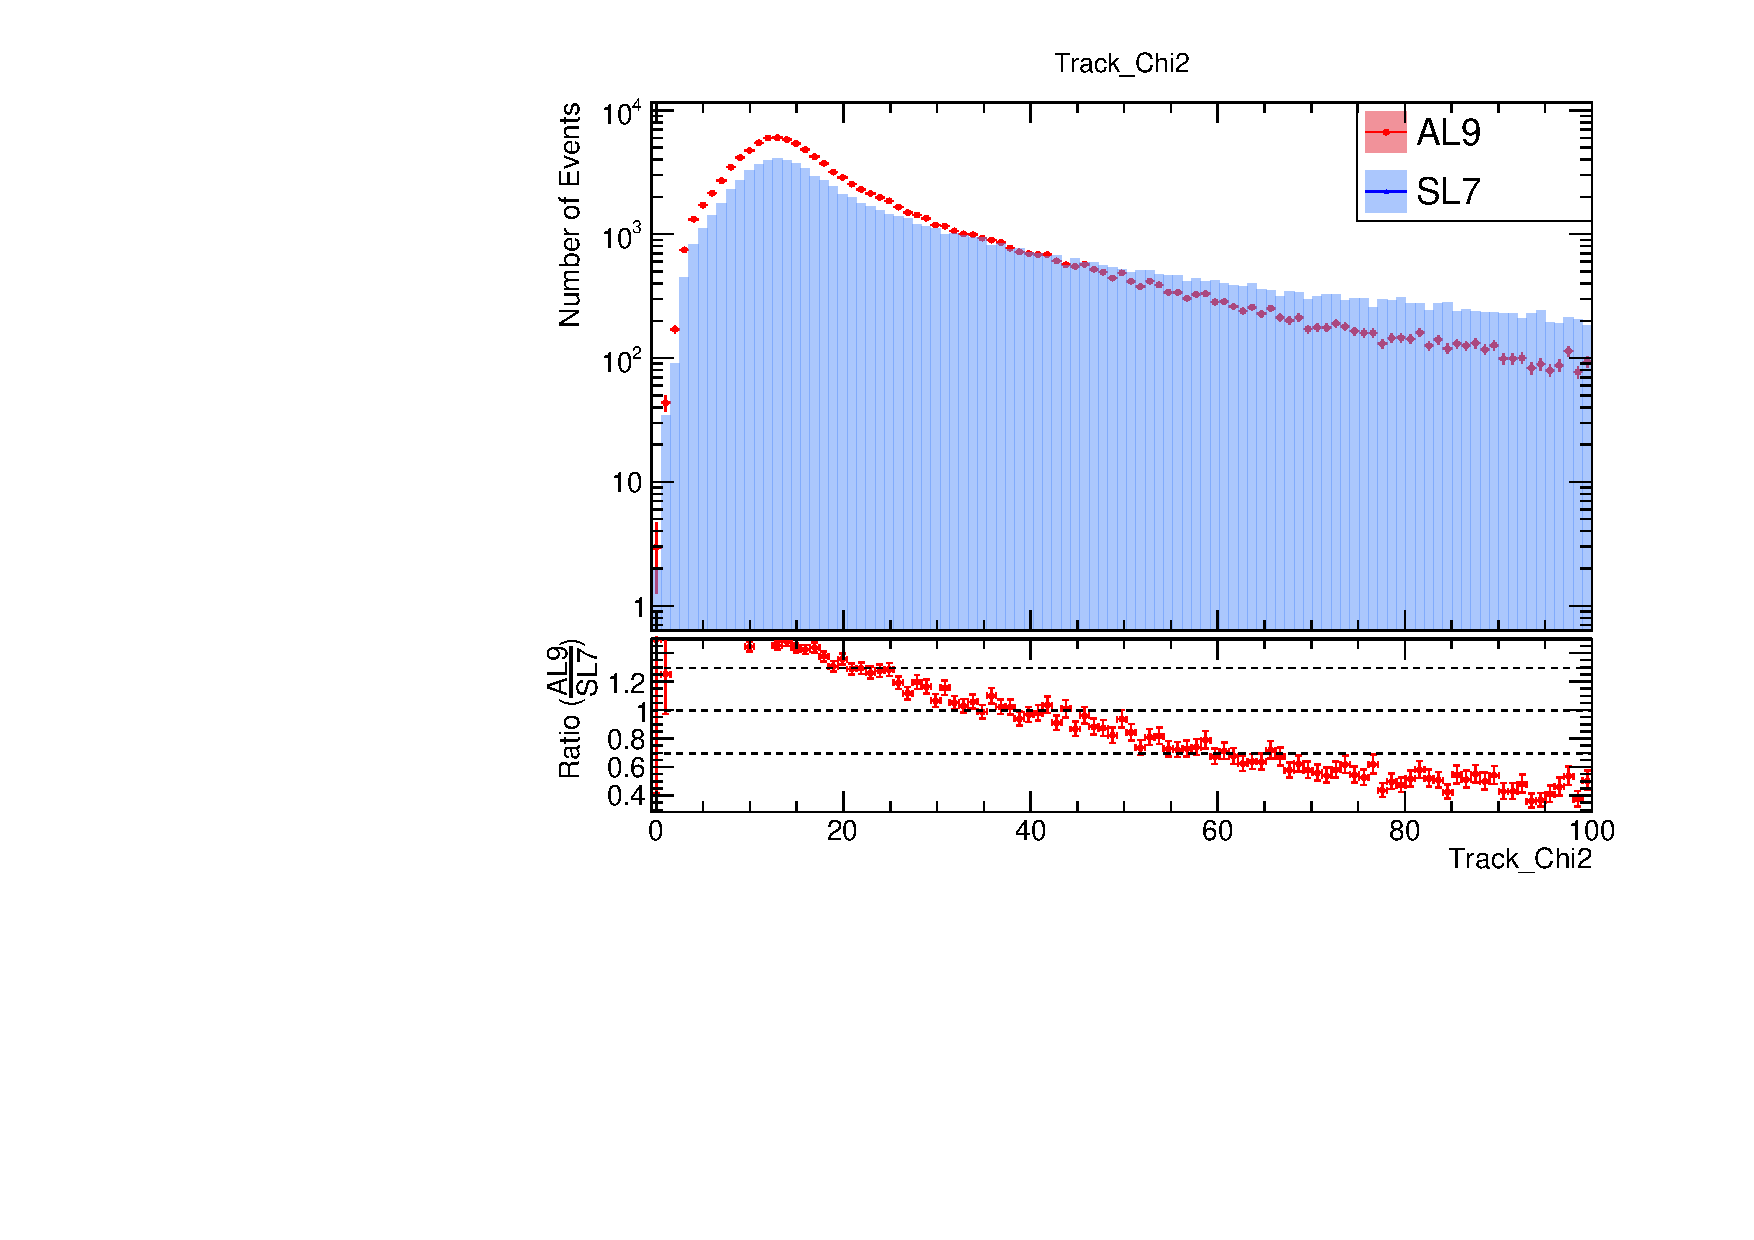
\includegraphics[width=\linewidth]{./output/Track_Chi2.pdf}
    \end{figure}
\end{frame}

\begin{frame}{Distribution of TrackChi2perDoF}
    \begin{figure}
        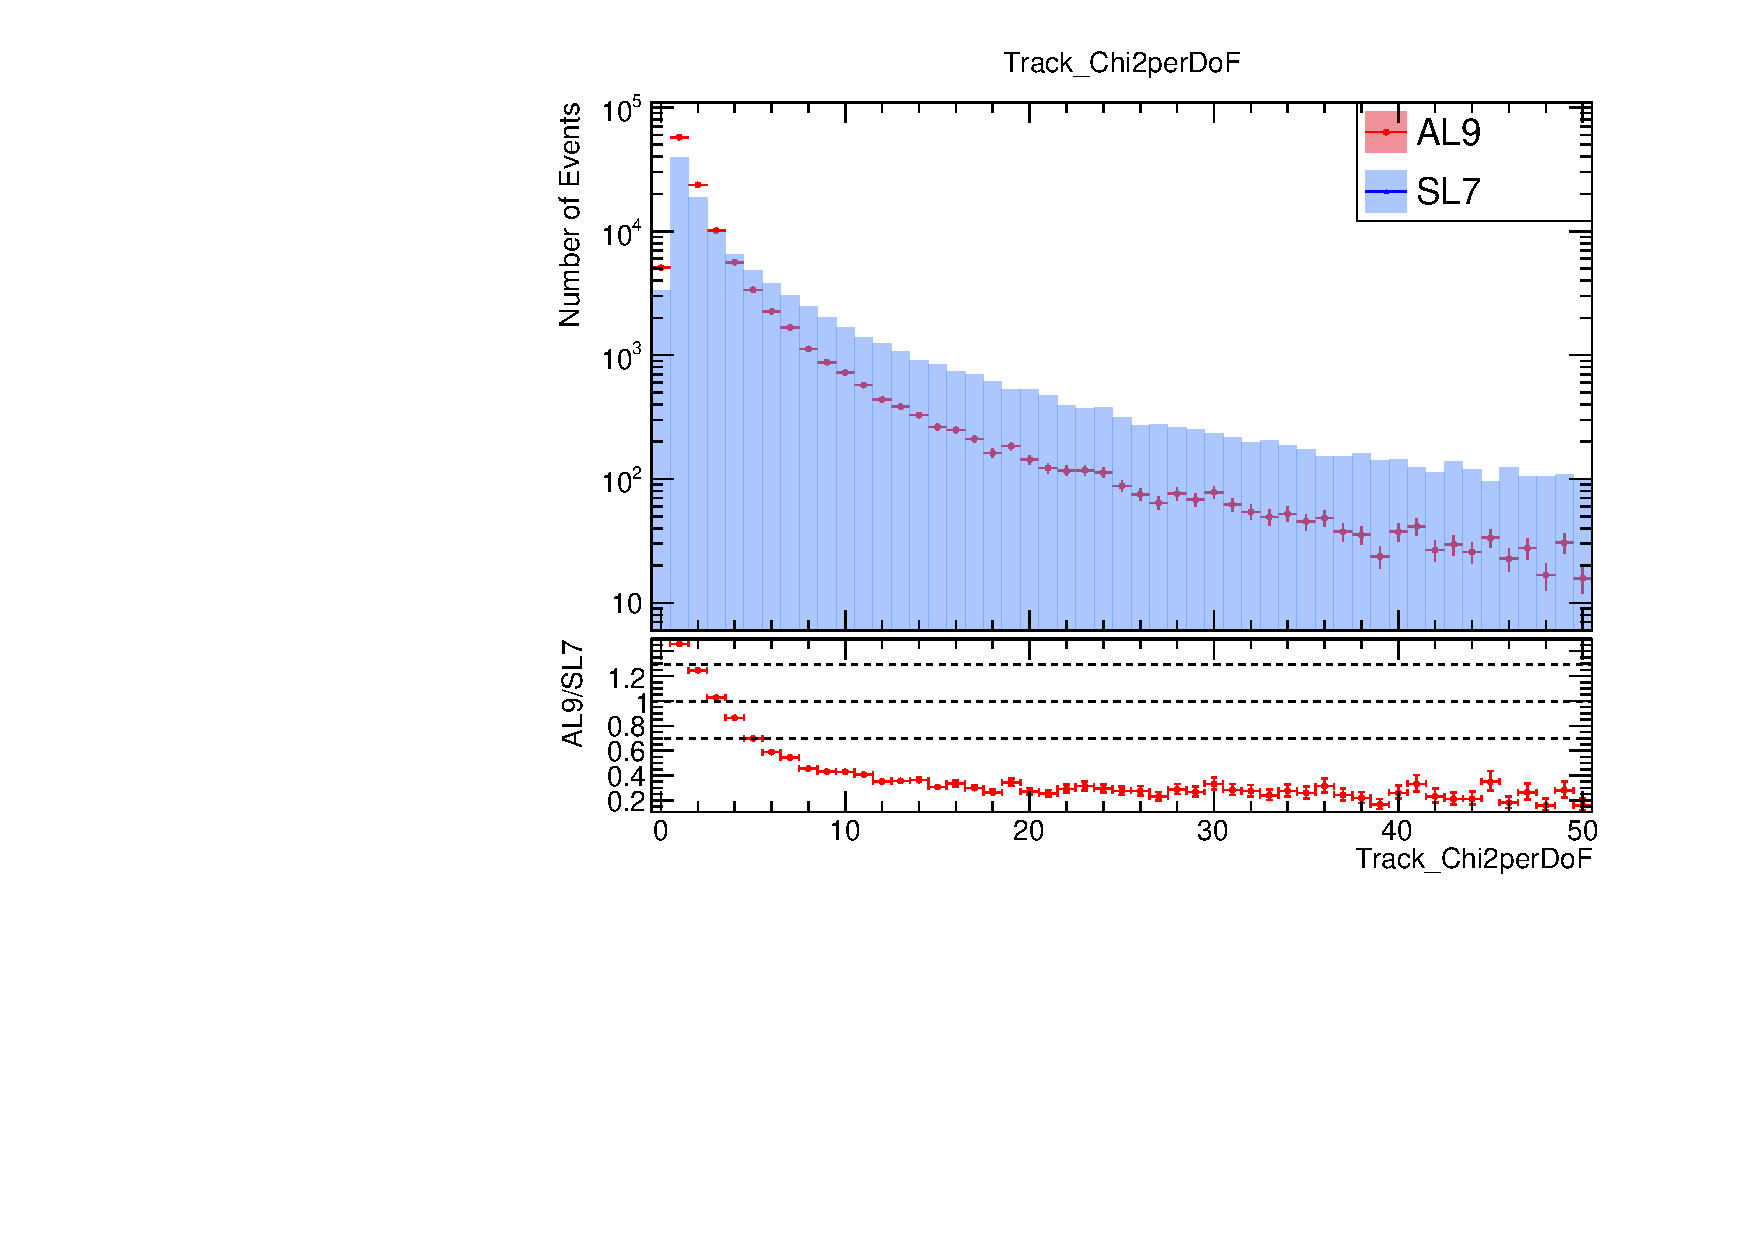
\includegraphics[width=\linewidth]{./output/Track_Chi2perDoF.pdf}
    \end{figure}
\end{frame}

\begin{frame}{Distribution of TrackNDoF}
    \begin{figure}
        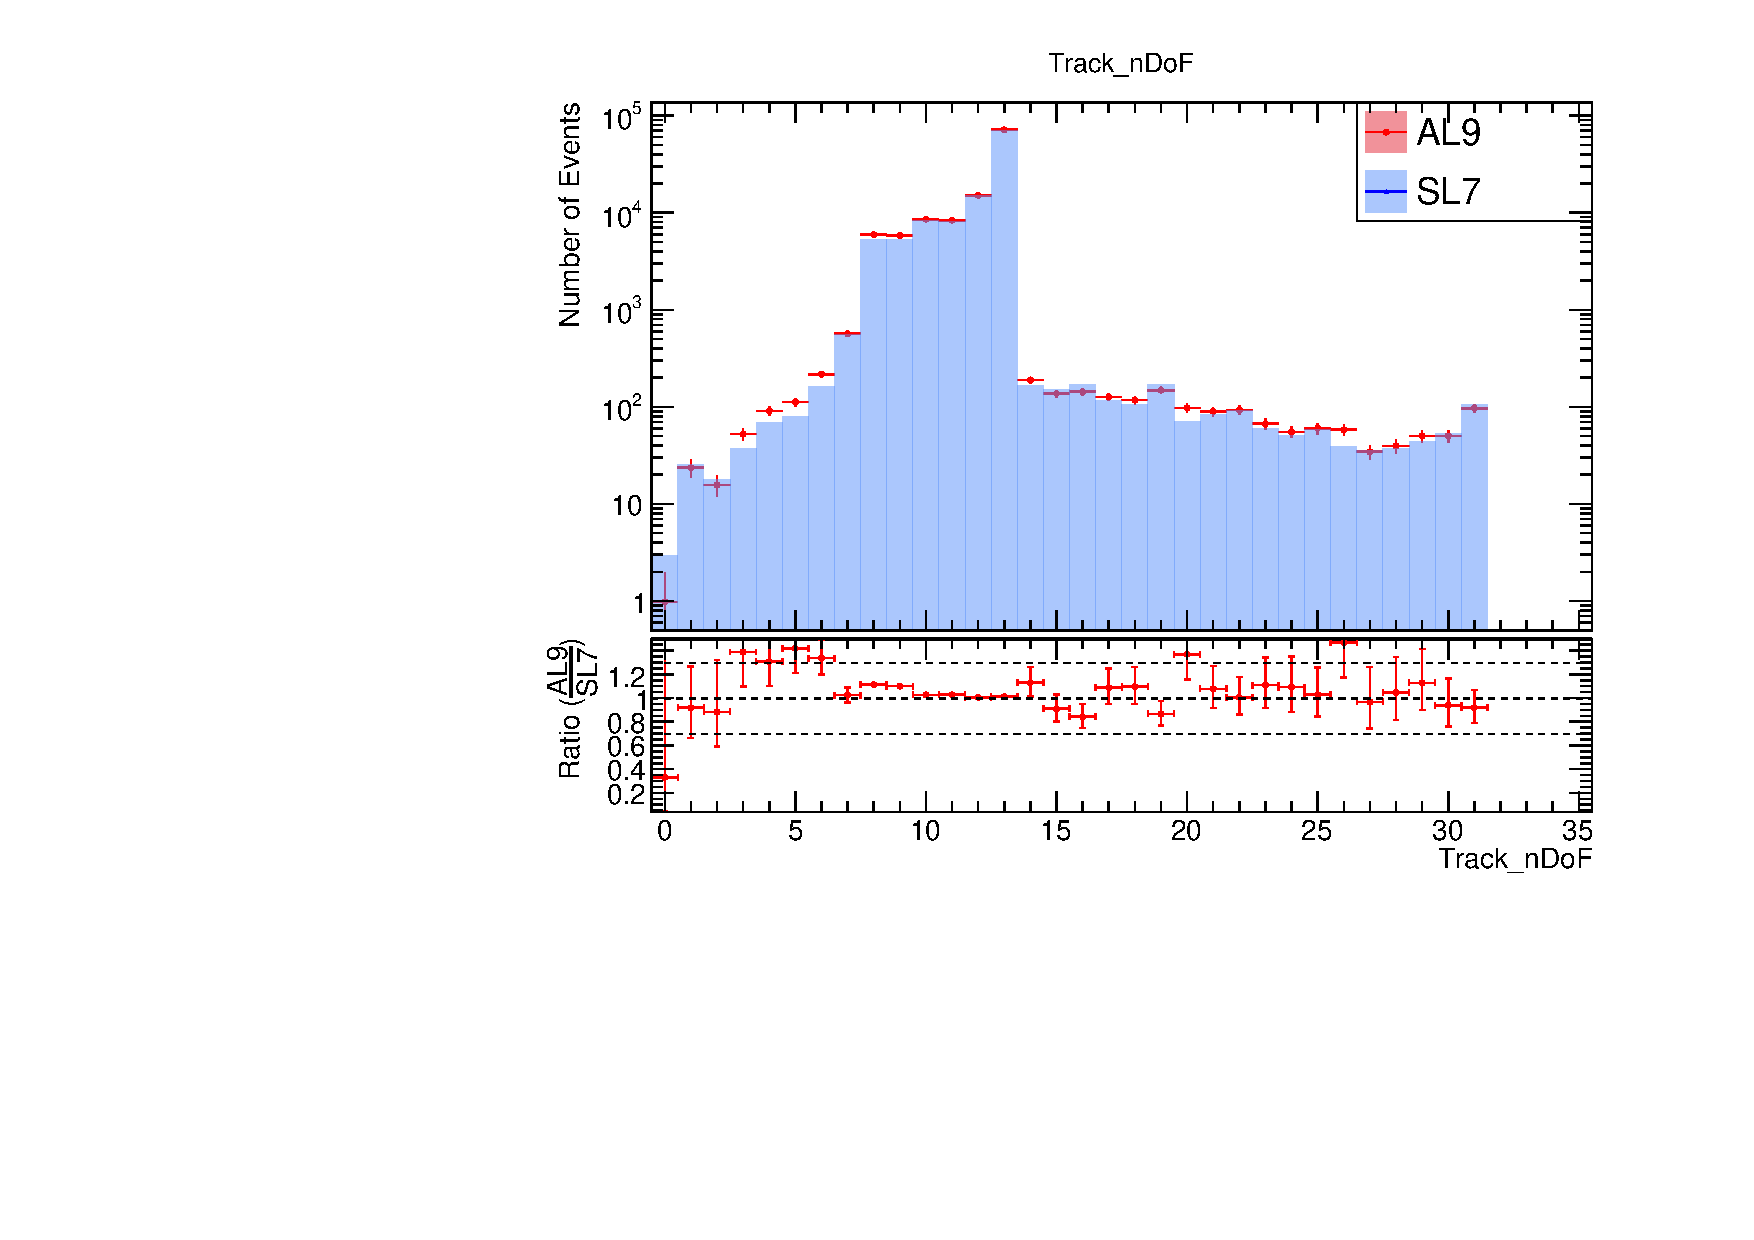
\includegraphics[width=\linewidth]{./output/Track_nDoF.pdf}
    \end{figure}
\end{frame}

\begin{frame}{Distribution of Track Charge}
    \begin{figure}
        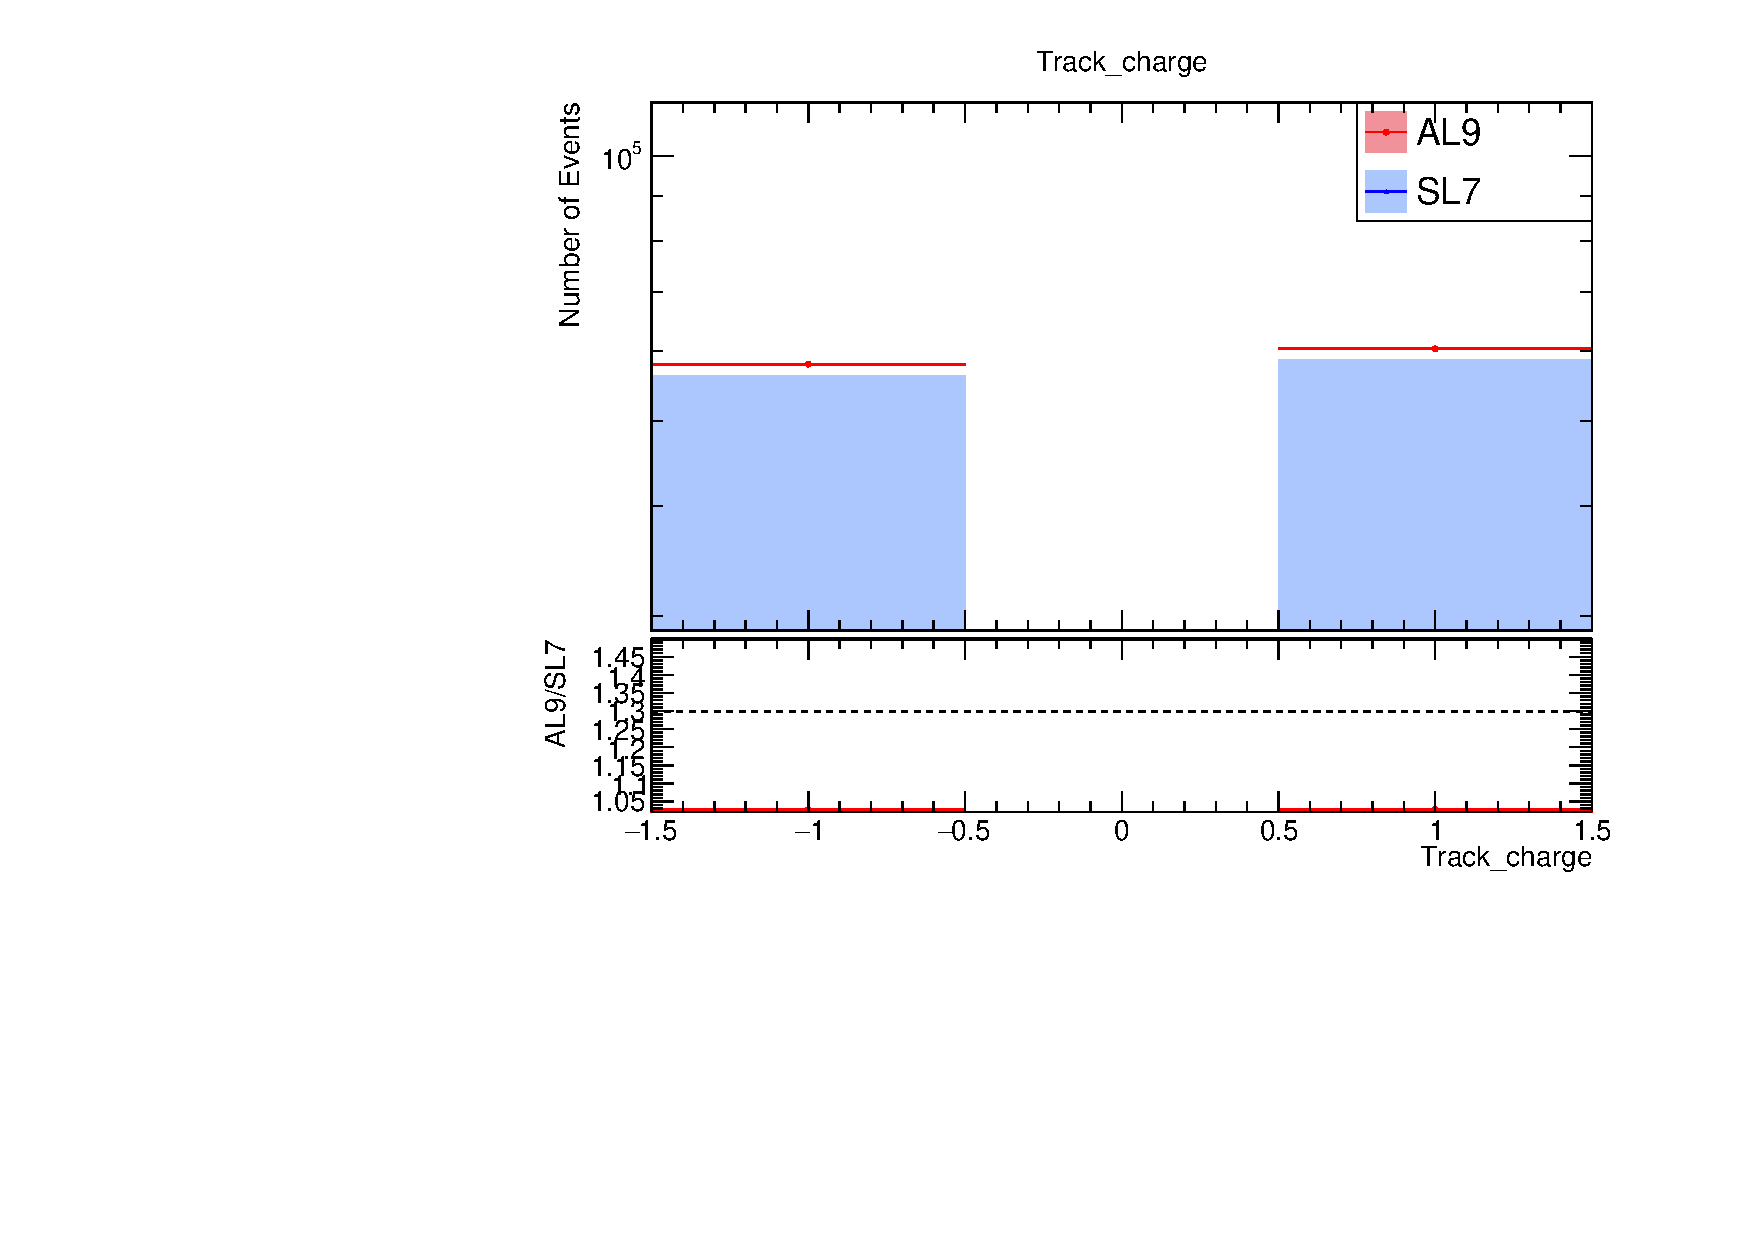
\includegraphics[width=\linewidth]{./output/Track_charge.pdf}
    \end{figure}
\end{frame}

\begin{frame}{Distribution of Track nLayers}
    \begin{figure}
        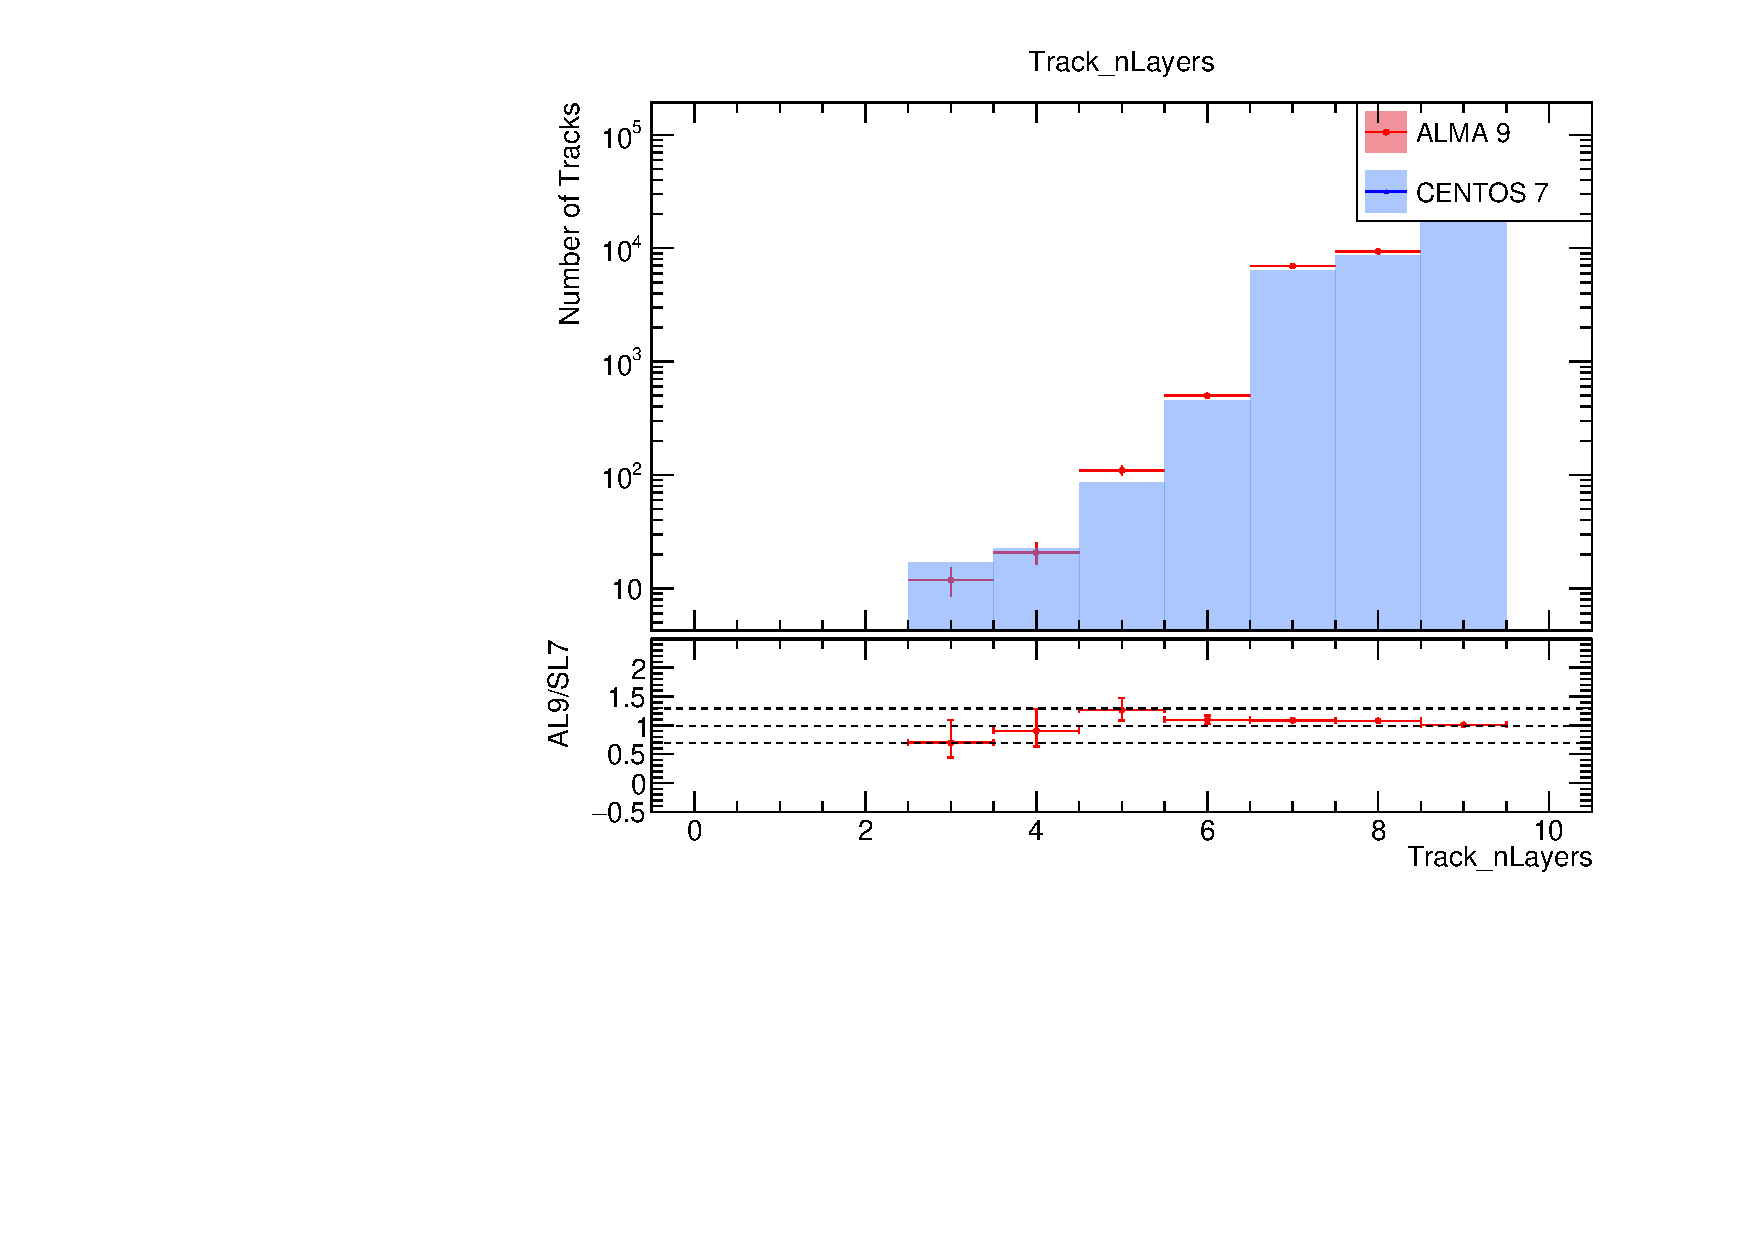
\includegraphics[width=\linewidth]{./output/Track_nLayers.pdf}
    \end{figure}
\end{frame}

\begin{frame}{Comments on Track Parameters}
    \begin{itemize}
        \item longTracks \> 5 is a mess, But not particularly useful
        \item Track Propagation Error is a easily interpretable function
        \item Track Chi2 changed a lot, much higher peak and lower tail in AL9, which is good.
        \item TrackNDoF shows good agreement except betweeen 3-5
        \item Track Charge in AL9 is slightly elevated, not sure why
        \item Track nLayers is also decent agreement except at 5-8
    \end{itemize}
\end{frame}